\subsection{Fluctuations of conserved charges} 
\label{sec:fluctuations}
\subsubsection{Physics introduction and observables}

In the phase diagram of strongly interacting matter at zero net baryon density, the presence of a chiral phase transition between hadronic matter and a QGP has been conjectured \cite{Pisarski:1983ms}, and arguments have been presented~\cite{Ejiri:2009ac,Ding:2018auz} in lQCD that the transition, for vanishing light quark masses, is of second order and belongs to the O(4) universality class. Due to the small but finite physical quark masses, in lQCD a rapid crossover is found \cite{Aoki:2006we,Aoki:2009sc,Borsanyi:2010bp,Bazavov:2011nk,Bhattacharya:2014ara} which, however, exhibits pseudo-critical features due to the smallness of the u- and d-quark masses and the proximity of the crossover region to the O(4) line \cite{Ejiri:2009ac,Ding:2013lfa}. 

In general, fluctuations can be linked to critical behaviour associated with a phase transition, and it has been pointed out that fluctuations of conserved charges in heavy-ion collisions can provide an experimental observable to test for critical behaviour in the phase diagram of strongly interacting matter \cite{Ejiri:2005wq,Bazavov:2017dus,Friman:2011pf,Bazavov:2012jq}. These fluctuations can be related to susceptibilities, specifically to the derivatives of the pressure with respect to the chemical potentials corresponding to the conserved charges. Here, the relevant `charges' are baryon number $B$, strangeness $S$, and electrical charge $Q$, and the corresponding chemical potentials are $\mu_B$, $\mu_S$, and $\mu_Q$. The susceptibilities are defined (see e.g. \cite{Bazavov:2012jq,Bellwied:2015lba}) in terms of dimensionless normalized chemical potentials \(\hat{\mu}_X\equiv \mu_X/T \) \: as

\begin{equation}
\chi_{ijk}^{BQS}(T) = \left.
\frac{\partial P(T,\hat{\mu})/T^4}{\partial\hat{\mu}_B^i \partial\hat{\mu}_Q^j \partial\hat{\mu}_S^k}\right|_{\hat{\mu}=0} \; .
\label{suscept}
\end{equation} 

\noindent The generalized susceptibilities can be computed in lQCD at vanishing chemical potential, exactly the conditions probed by experiments at the LHC. Within the Grand Canonical Ensemble (GCE), these generalized susceptibilities can be related to experimental measurements of the fluctuations of particle multiplicities, such as the net number of baryons. For instance, a measurement of higher moments or cumulants of net baryon number in relativistic nuclear collisions can be directly related \cite{Karsch:2010ck,Skokov:2012ds,Karsch:2012wm,Karsch:2017mvg,Borsanyi:2013hza,Borsanyi:2014ewa} to theoretical predictions from lQCD or from more phenomenological models of the chiral phase transition \cite{Almasi:2017bhq,Parotto:2018pwx} to shed light on the possible critical behaviour near the QCD phase boundary. 
For a distribution of the net baryon number, $\Delta N_B = N_B - N_{\overline{B}}$, with moments defined as 

\begin{equation}
\mu_i = \langle (\Delta N_B - \langle \Delta N_B \rangle )^i \rangle ,
\end{equation}
the cumulants $\kappa_i$ can be directly linked to the generalized susceptibilities such as

\begin{equation}
\kappa_2 = \mu_2 = VT^3 \chi_2^B
\end{equation}
\begin{equation}
\kappa_3 = \mu_3 = VT^3 \chi_3^B  
\end{equation}
\begin{equation}
\kappa_4 = \mu_4 - 3\mu_2^2 = VT^3 \chi_4^B.
\end{equation}


\begin{figure}[ht]
\begin{center}
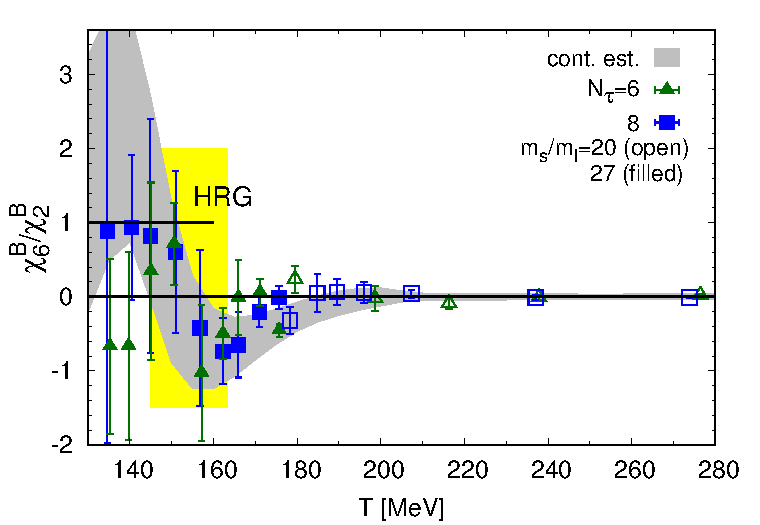
\includegraphics[width=0.45\textwidth]{\main/lightflavour/figs/B6_B2_wideT_27.pdf}
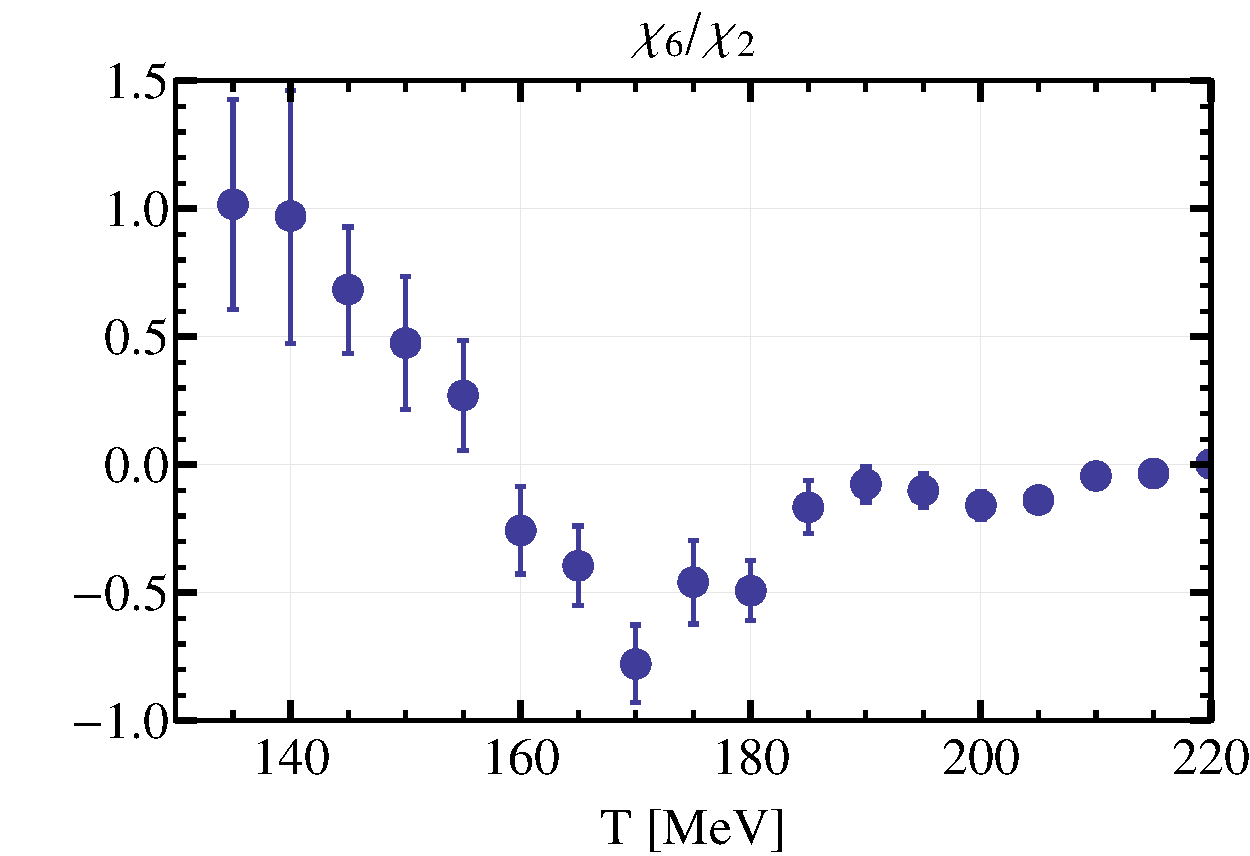
\includegraphics[width=0.46\textwidth]{\main/lightflavour/figs/c6c2_fromLattice.pdf}
\end{center}
\caption{Ratio of sixth to second-order baryon number susceptibilities from lQCD. The left-hand figure is from \cite{Bazavov:2017dus}. The right-hand figure is calculated from recent lQCD data on  sixth and  second  order susceptibilities from \cite{Borsanyi:2018grb}. }  
\label{fig:chi62}
\end{figure}

In the O(4) universality class, a singular contribution to the pressure shows up for higher order  moments.
More specifically, at vanishing chemical potential, all odd susceptibilities of the net baryon number vanish.  
In addition, in the O(4) universality class, the second- and fourth-order susceptibilities remain finite  at  the  phase  transition  temperature  at $\mu_B~=~0$  in  the  chiral  limit,
implying  that  only  sixth-  and  higher-order  susceptibilities  diverge \cite{Ejiri:2005wq,Friman:2011pf}. Thus, for  physical  quark  masses and at $\mu_B~=~0$, only higher order cumulants $\kappa_n$ with $n\geq 6$ can exhibit O(4) criticality,  whereas at finite $\mu_B$ this is already the case for $\kappa_n$ with $n\geq 3$.  

Sensitivity to chiral criticality due to the vicinity of the O(4) line at $\mu_B~=~0$ is borne out in phenomenological models as is shown in \cite{Friman:2011pf,Almasi:2017bhq}, and in lQCD predictions \cite{Bazavov:2017dus,Borsanyi:2018grb}, by strong deviations of $\chi_6^B/\chi_2^B$ from unity as shown in Fig.~\ref{fig:chi62}.

We note that a convenient baseline for the cumulants of multiplicity distributions and fluctuations of produced particles in relativistic nuclear collisions can be obtained in the framework of the hadron re\-so\-nance gas (HRG) \cite{Allton:2005gk,Karsch:2010ck,BraunMunzinger:2011ta,Borsanyi:2018grb,Luo:2017faz}. In this model, uncorrelated Poissonian fluctuations of baryon and anti-baryon multiplicities result in a Skellam distribution for the net baryon number, in which the higher moments and cumulants can all be related to the first moments in the following way \cite{BraunMunzinger:2011ta,BraunMunzinger:2011dn, Braun-Munzinger:2018yru}:
\begin{equation}
\label{lbaseline}
\kappa_n(N_B - N_{\overline{B}}) = \langle (N_B +(-1)^n N_{\overline{B}}) \rangle
\end{equation}
For zero net baryon number then all odd cumulants vanish and all even cumulants are identical.

Measuring such cumulants with precision poses a formidable experimental challenge due to the requirement of very large data sets ($> 10^9$ events of a particular event or centrality class) with superb control of systematic uncertainties. As a first physics case to consider along this line, the impact of measuring the distribution of net protons as a proxy for net baryons needs to be studied further. We note that, at LHC energy and low transverse momentum, particle production near mid-rapidity takes place mostly in gluonic processes, implying that isospin asymmetries, as in the colliding nuclei, are absent. As a consequence, the production yields of protons and neutrons should be very close. For light nuclei this isospin symmetry has been checked experimentally, albeit with significant uncertainties. 
In addition, non-critical contributions to the cumulants from volume fluctuations and global baryon number conservation \cite{Skokov:2012ds,Braun-Munzinger:2016yjz, Braun-Munzinger:2018yru} need to be evaluated and the data corrected accordingly. Furthermore, in particular for comparison to lQCD predictions, care needs to be taken to keep experimental cuts such as in \pT\ to a minimum insofar as such cuts cannot be introduced in lQCD \cite{Karsch:2015zna,Alba:2015iva}.
     
Two-particle correlations with net baryons can also be used to explore transport properties of the hydrodynamic evolution. The baryon diffusion constant $D$ is a fundamental transport property of the quark-gluon plasma, similar to shear viscosity $\eta$ or bulk viscosity $\zeta$. It characterizes the mobility of baryon number, and is predicted to be finite at the LHC despite the fact that $\mu_{B}\sim0$. A two-particle correlation function as been proposed~\cite{Floerchinger:2015efa}, which explores correlations of net-baryon fluctuations as a function of separations in azimuthal angle and rapidity, and can provide experimental constraints on the diffusion coefficient $D$. As $\mu_{B}\sim0$ at the LHC, such an analysis has yet to be carried out in Run 1 and 2 data since it is statistically challenging, and will be greatly aided by the increase by about a factor 100 in the \PbPb integrated luminosity foreseen for Runs 3 and 4.

\subsubsection{State of the art experimental measurements and present limitations}

Net proton fluctuations measured by the ALICE experiment and in the STAR beam energy scan program provide interesting and stimulating results. The measurements at STAR~\cite{Adamczyk:2013dal} complement the corresponding measurements from ALICE, which will make it possible to pin down the global structure of the phase diagram of strongly interacting matter in a wide range of temperatures and net-baryon densities. However, before drawing firm conclusions by confronting theoretical calculations with  data, non-dynamical contributions stemming from unavoidable fluctuations of  participant nucleons and  overall baryon number conservation have to be subtracted from the experimental measurements. Both of these non-dynamical contributions, which exist neither in lQCD nor in the HRG model, lead to deviations from the baseline as defined in Eq.~\ref{lbaseline}. Indeed, the acceptance dependence of the second-order cumulants of net-protons measured by ALICE~\cite{Rustamov:2017lio} exhibits deviations from the non-critical (Skellam) baseline. However, these deviations were explained by global baryon number conservation~\cite{Rustamov:2017lio, Braun-Munzinger:2016yjz, Braun-Munzinger:2018yru}, which, in accordance with the experimental findings, decreases the amount of fluctuations with the increasing acceptance. This is the first experimental verification of the lQCD predictions for the second-order cumulants of net-baryon distributions. This also serves as a strong support of the HRG model, in that experimental measurements of the second cumulants of net-protons do not show any evidence of criticality and actually coincide with the second cumulants of the Skellam distribution.  In order to probe critical phenomena, higher cumulants beyond the second order have to be addressed. 

As mentioned in the previous section, even at vanishing net-baryon densities, lQCD and other theoretical calculations such as Polyakov-loop extended Quark- Meson model (PQM)~\cite{Almasi:2017bhq} predict critical fluctuations encoded in the deviations of net-baryon $\kappa_{4}/\kappa_{2}$ and $\kappa_{6}/\kappa_{2}$ from unity. Moreover, at the pseudo critical temperature of about 156 MeV the magnitudes of $\kappa_{4}/\kappa_{2}$ and $\kappa_{6}/\kappa_{2}$  are predicted in Ref.~\cite{Almasi:2017bhq} to be 0.5 and -0.39, respectively. Similar values of $\kappa_{6}/\kappa_{2}$ are quoted in different lQCD calculations as presented in Fig~\ref{fig:chi62}.  These numbers, shown in  Fig.~\ref{netpALICE_STAR}, do not take into account experimental artefacts such as global net-baryon number conservation and unavoidable fluctuations of participating nucleons from event to event. Also shown are the values of of $\kappa_{4}/\kappa_{2}$ and $\kappa_{6}/\kappa_{2}$ after accounting for these non-dynamical effects using the procedure in Refs.~\cite{Braun-Munzinger:2016yjz, Braun-Munzinger:2018yru}. Even after accounting for participant fluctuations and global baryon number conservation we observe deviations in $\kappa_{4}/\kappa_{2}$ and $\kappa_{6}/\kappa_{2}$ from unity, although they are somewhat reduced.   This motivates our experimental program  of measuring higher moments of net-proton distributions at the LHC energies. Also, fluctuation measurements  are underway in the strange baryon sector to approach measurements of net baryon number fluctuations. All this will be greatly helped by the anticipated dramatic increase in statistics in Runs 3 and 4.

\begin{figure}[ht]
\begin{center}
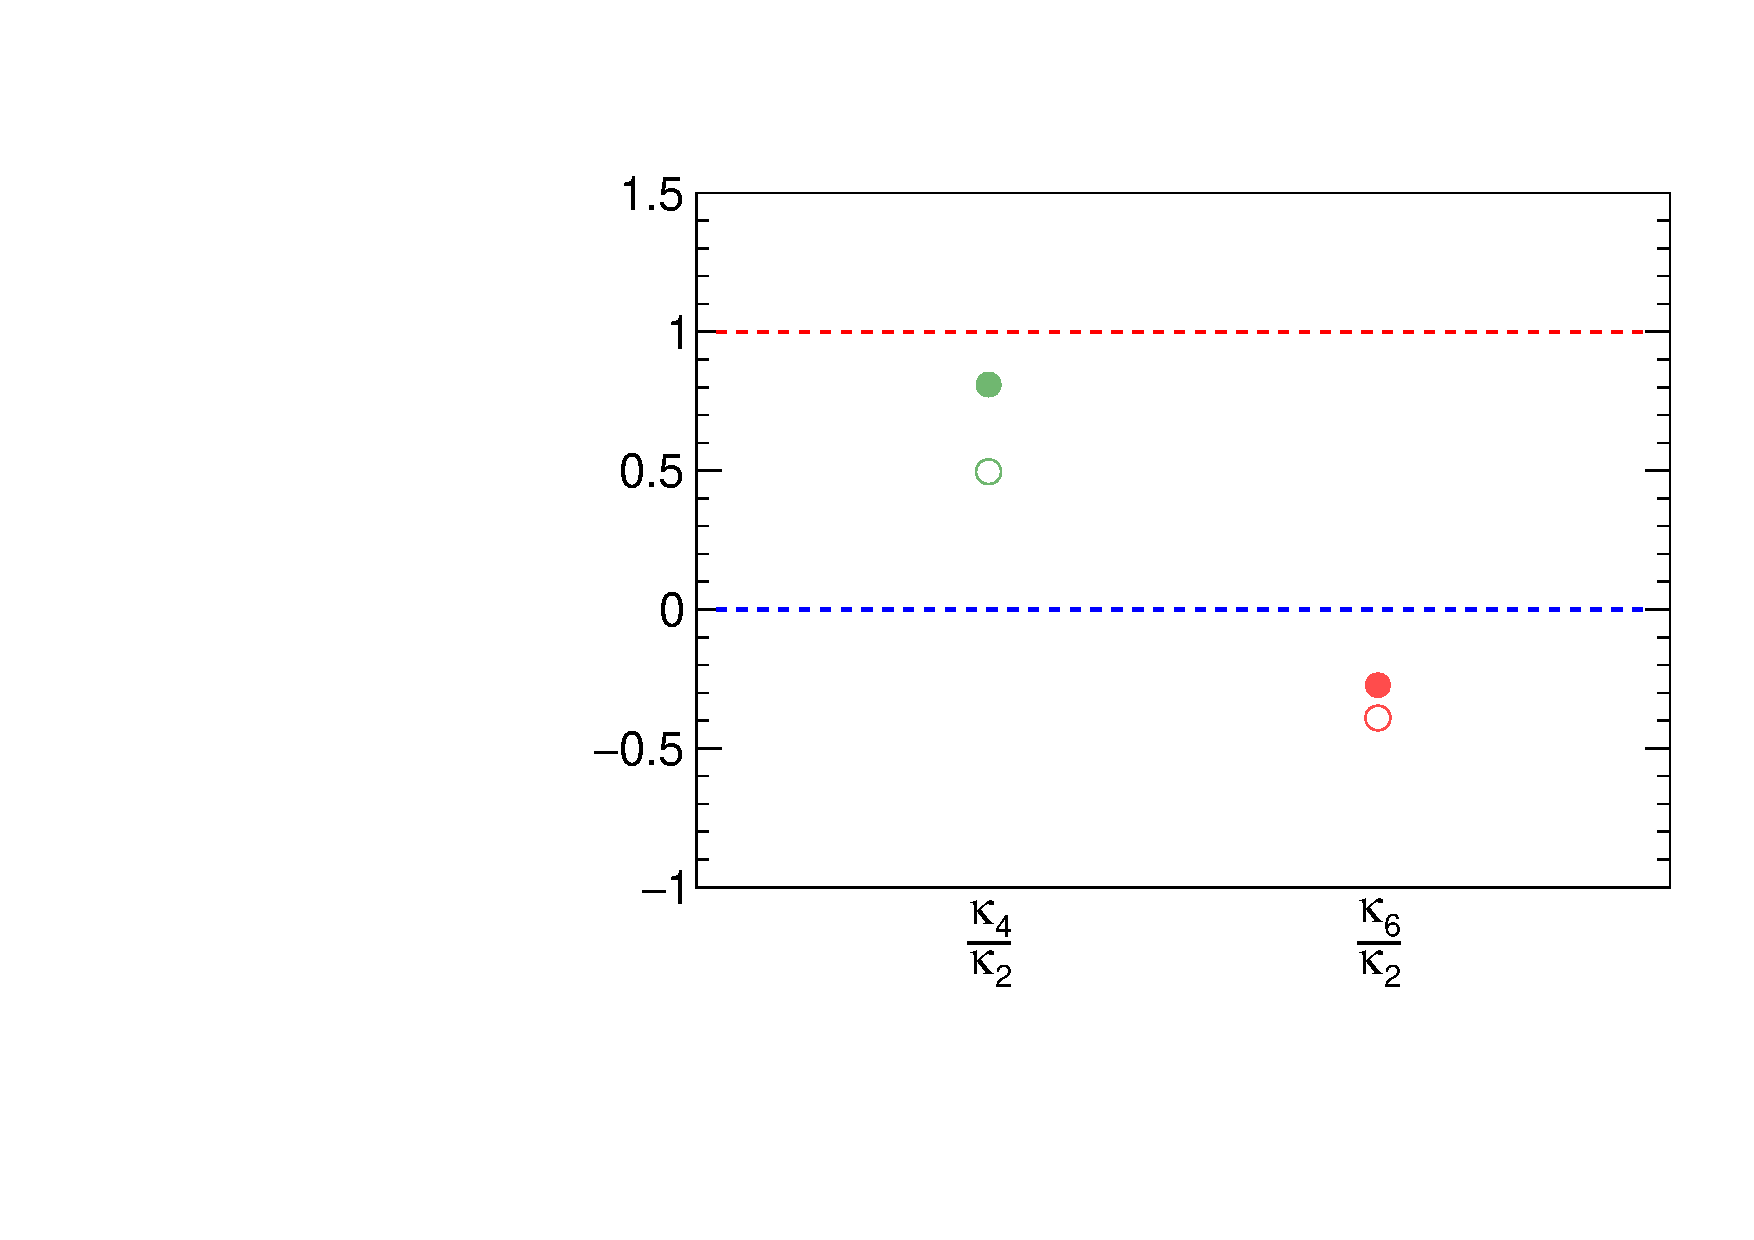
\includegraphics[width=0.6\textwidth]{\main/lightflavour/figs/baseLine.pdf}
\end{center}
\caption{$\kappa_{4}/\kappa_{2}$ and $\kappa_{6}/\kappa_{2}$  as calculated within PQM~\cite{Almasi:2017bhq} model (open symbols).  After taking into account contributions from participant nucleon fluctuations and global baryon number conservation~\cite{Braun-Munzinger:2016yjz, Braun-Munzinger:2018yru}, the deviations from unity decrease (closed symbols).} 
\label{netpALICE_STAR}
\end{figure}

\subsubsection{Projections for HL-LHC}

As discussed above, precise studies of the higher-order cumulants of particle multiplicity distributions are needed to verify theoretical predictions. In this section we estimate the statistics needed to address these measurements with the ALICE experiment. For this purpose two distinct  Monte Carlo simulations have been developed. In the first approach, following recent developments in~\cite{Bzdak:2018axe}, the probability distribution function of net-protons is approximated  by a superposition of two Gaussian distributions which has four free parameters. Using the experimentally measured second cumulant of net-protons for 0-5 \% most central \PbPb collisions~\cite{Rustamov:2017lio} and the $\kappa_{4}/\kappa_{2}$ and $\kappa_{6}/\kappa_{2}$ ratios from the PQM model~\cite{Almasi:2017bhq}, we first obtained absolute values for $\kappa_{4}$ and $\kappa_{6}$.  These values were adjusted to account for fluctuations from participant nucleons in 0-5$\%$ most central \PbPb collisions and global baryon number conservation~\cite{Braun-Munzinger:2016yjz, Braun-Munzinger:2018yru}. Finally, the free parameters of the double Gaussian distribution were fixed using the expected values of $\kappa_{1}$ , $\kappa_{2}$ , $\kappa_{4}$ and $\kappa_{6}$ , where $\kappa_{1}$ equals zero by definition. The event-by-event net-proton number was sampled from the double Gaussian function  thus generating the net-proton distribution for a given number of events. 
In the second approach the probability distribution functions of protons and anti-protons are calculated separately by exploiting the Pearson curve method \cite{Behera:2017xwg}. This approach also needs four measurements as inputs, which are taken as the first four cumulants of the proton and anti-proton multiplicities measured by ALICE (presented in \cite{Behera:2018wqk}).  The net-proton distribution for a given number of events is constructed by sampling the obtained proton and anti-proton probability distribution functions. 
In each approach, the resulting statistical uncertainties are obtained using the subsample method.  

The obtained results for $\kappa_{4}/\kappa_{2}$ and $\kappa_{6}/\kappa_{2}$ and their corresponding statistical uncertainties are shown in Fig.~\ref{fig:c4c2toymc} as a function of the simulated event statistics. The dashed red lines correspond to the input values predicted by PQM calculations of critical fluctuations (CF) and assuming a double Gaussian net-proton distribution, while the green dashed lines come from the Pearson curve method based on the lower-order cumulants measured by ALICE. As expected, with increasing statistics both $\kappa_{4}/\kappa_{2}$ and $\kappa_{6}/\kappa_{2}$ approach their nominal values. The statistics necessary to measure these cumulants are presented in the bottom panels of Fig.~\ref{fig:c4c2toymc}, where the deviations of the expected values from unity are quantified in terms of the magnitudes of the statistical uncertainty ($\sigma$). As seen from the left panel of Fig.~\ref{fig:c4c2toymc}, for $\kappa_{4}/\kappa_{2}$ already 10 million events are sufficient to distinguish the expected critical fluctuations signal from unity with a statistical significance of $4\sigma$. Similar conclusions are obtained with the Pearson curve method.  Several times this amount of data has already been recorded by ALICE, and the expected statistics in Run 3 and Run 4 will make it possible to measure  $\kappa_{4}/\kappa_{2}$ with unprecedented precision.  

For $\kappa_{6}/\kappa_{2}$, however, significantly larger event statistics is needed. As seen from the right panel of Fig.~\ref{fig:c4c2toymc}, more than 5 billion events generated with the double Gaussian approach is needed in order to observe statistically significant deviations from unity in favor of the critical values indicated with the red dashed line. Moreover, results obtained with the Pearson curve method indicate that more than 200 million events would be sufficient in order to claim a significant deviation from unity in favor of the corresponding expected value. This inconsistency in the estimation of the required statistics for $\kappa_{6}/\kappa_{2}$ comes mainly from the different baseline values of -1.43 and -0.27 used in the Pearson and double Gaussian methods, respectively. In addition, the value of $\kappa_{2}$ used in the Pearson method is about two times smaller than measured in the experiment and used in the double Gaussian method. However, both methods indicate that the amount of data to be recorded in Runs 3 and 4 should be sufficient to probe the critical phenomena contained in $\kappa_{6}/\kappa_{2}$. 
      
\begin{figure}[ht]
\begin{center}$
\begin{array}{cc}
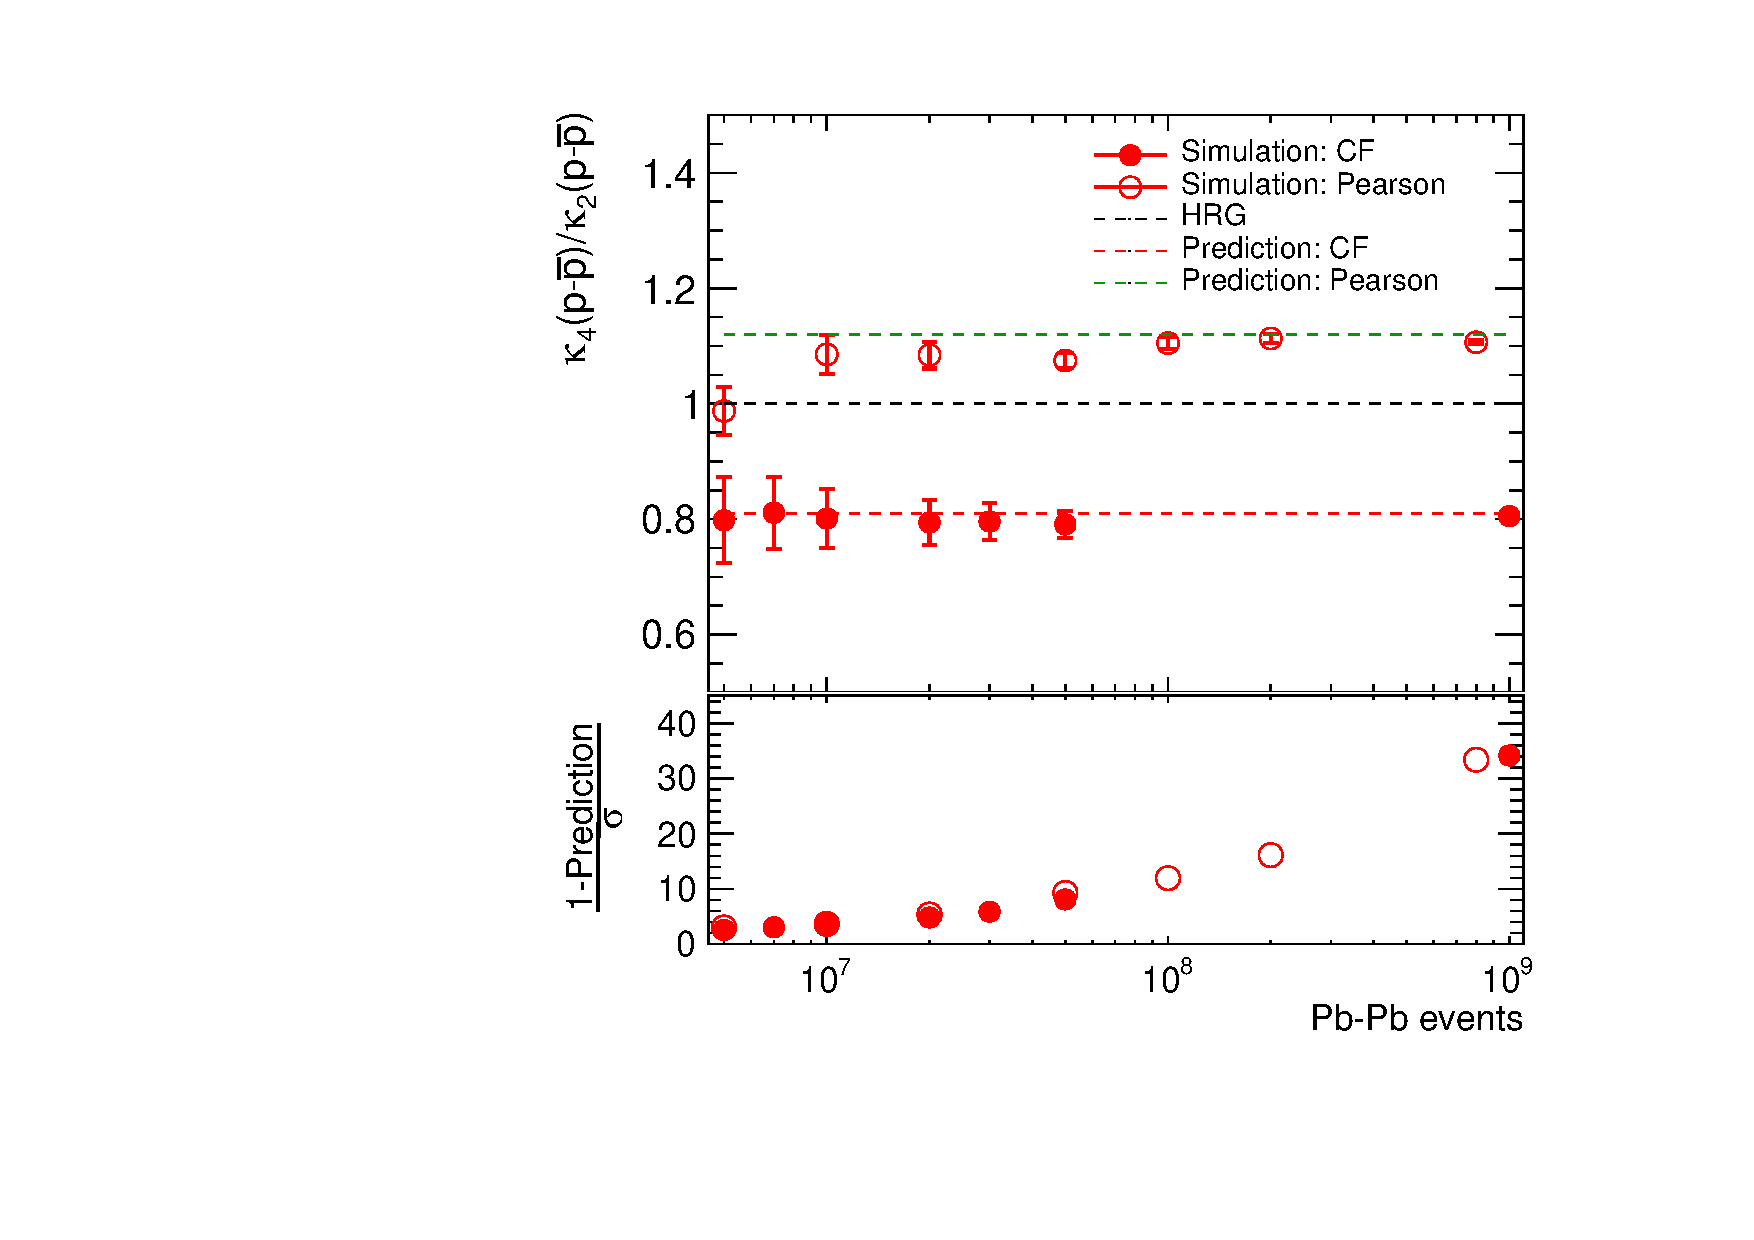
\includegraphics[width=0.45\textwidth]{\main/lightflavour/figs/stat42.pdf} &
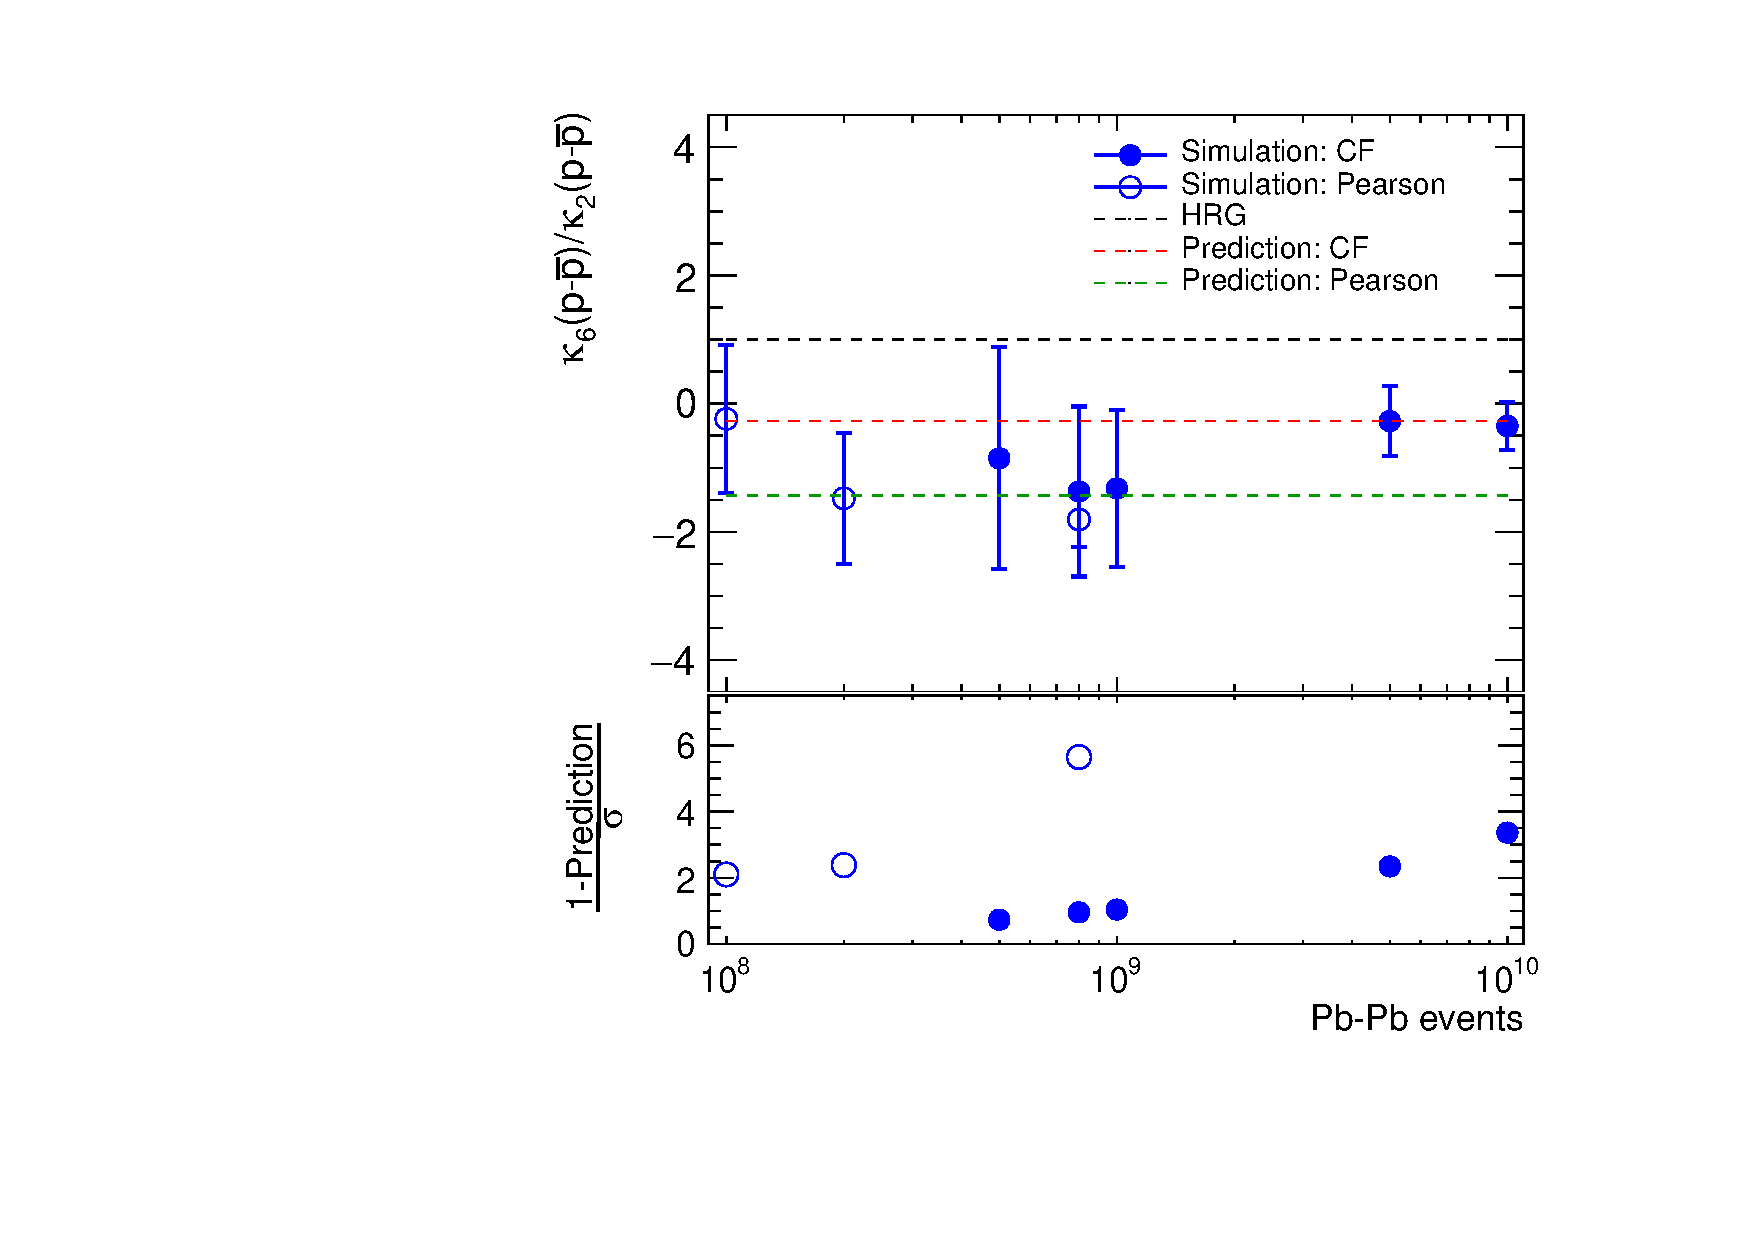
\includegraphics[width=0.45\textwidth]{\main/lightflavour/figs/stat62.pdf}
\end{array}$
\end{center}
\caption{Simulated values of  $\kappa_{4}/\kappa_{2}$ (left panel) and $\kappa_{6}/\kappa_{2}$ (right panel) as functions of the generated number of events. Full symbols represent results obtained with the double Gaussian approach adjusted to reproduce critical fluctuations (CF) predicted in the PQM model~\cite{Almasi:2017bhq}. Open symbols are obtained with the Pearson Curve Method\cite{Behera:2017xwg}.}
\label{fig:c4c2toymc}
\end{figure}



